\documentclass[12pt]{article}
\usepackage[utf8]{inputenc}
\usepackage{tgbonum}
\usepackage[a4paper, total={7in, 10in}]{geometry}
\usepackage{graphicx}
\usepackage{minted}
\title{Lab Assignment 2}
\author{Akshat Mittal - 20107}
\date{May 2021}
\begin{document}
\maketitle
\vspace{7mm}
\textbf{Contents}
\vspace{7mm}
\begin{enumerate}
    \item Calculator
    \item Leap year
    \item Tax calculator
    \item Signum function
    \item Height calculator
    \item Temperature measurement
    \item Triangle and its sides
    \item Number name
    \item Electricity Bill
    \item Reversing a 5-digit number
\end{enumerate}
\newpage
\section{}
\subsection{Flowchart}
\begin{figure}[h]
    \centering
    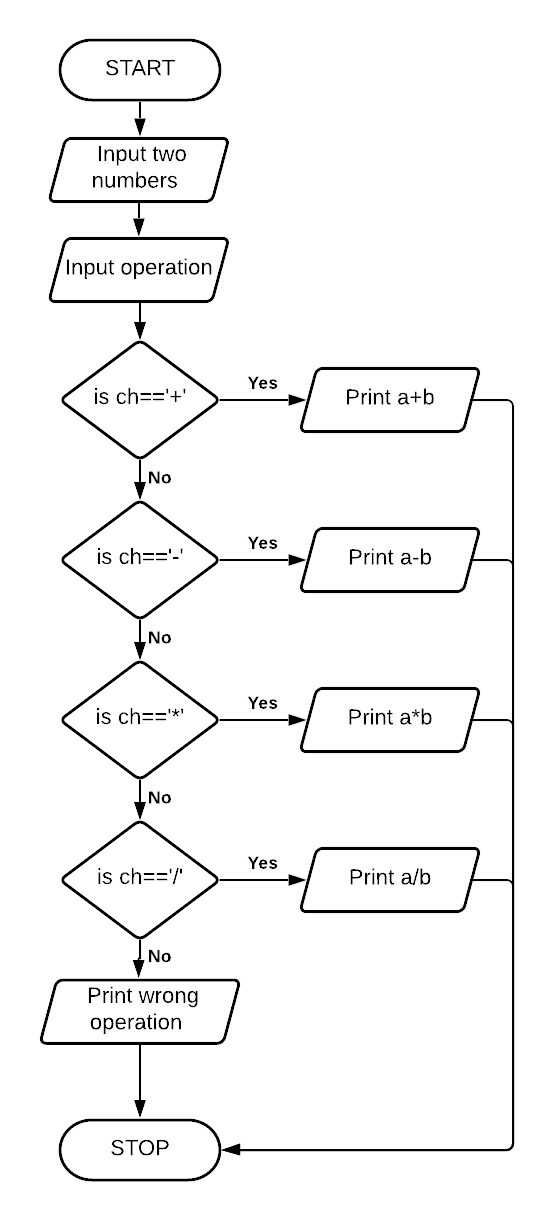
\includegraphics[width=0.5\textwidth]{Flowchart01.png}
\end{figure}
\newpage
\subsection{Code}
\inputminted{c}{q1.c}
\subsection{Output}
\begin{figure}[h]
    \centering
    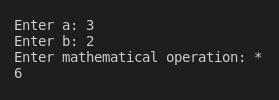
\includegraphics{1.png}
\end{figure}
\newpage
\section{}
\subsection{Flowchart}
\begin{figure}[h]
    \centering
    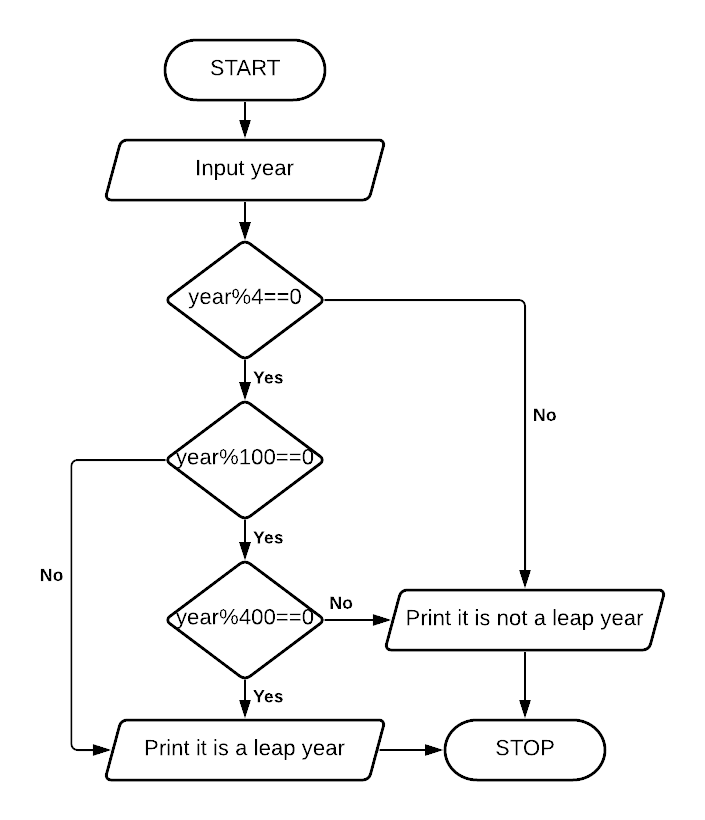
\includegraphics[width=0.8\textwidth]{Flowchart02.png}
\end{figure}
\newpage
\subsection{Code}
\inputminted{c}{q2.c}
\subsection{Output}
\begin{figure}[h]
    \centering
    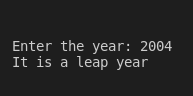
\includegraphics[width=0.5\textwidth]{2.png}
\end{figure}
\newpage
\section{}
\subsection{Flowchart}
\begin{figure}[h]
    \centering
    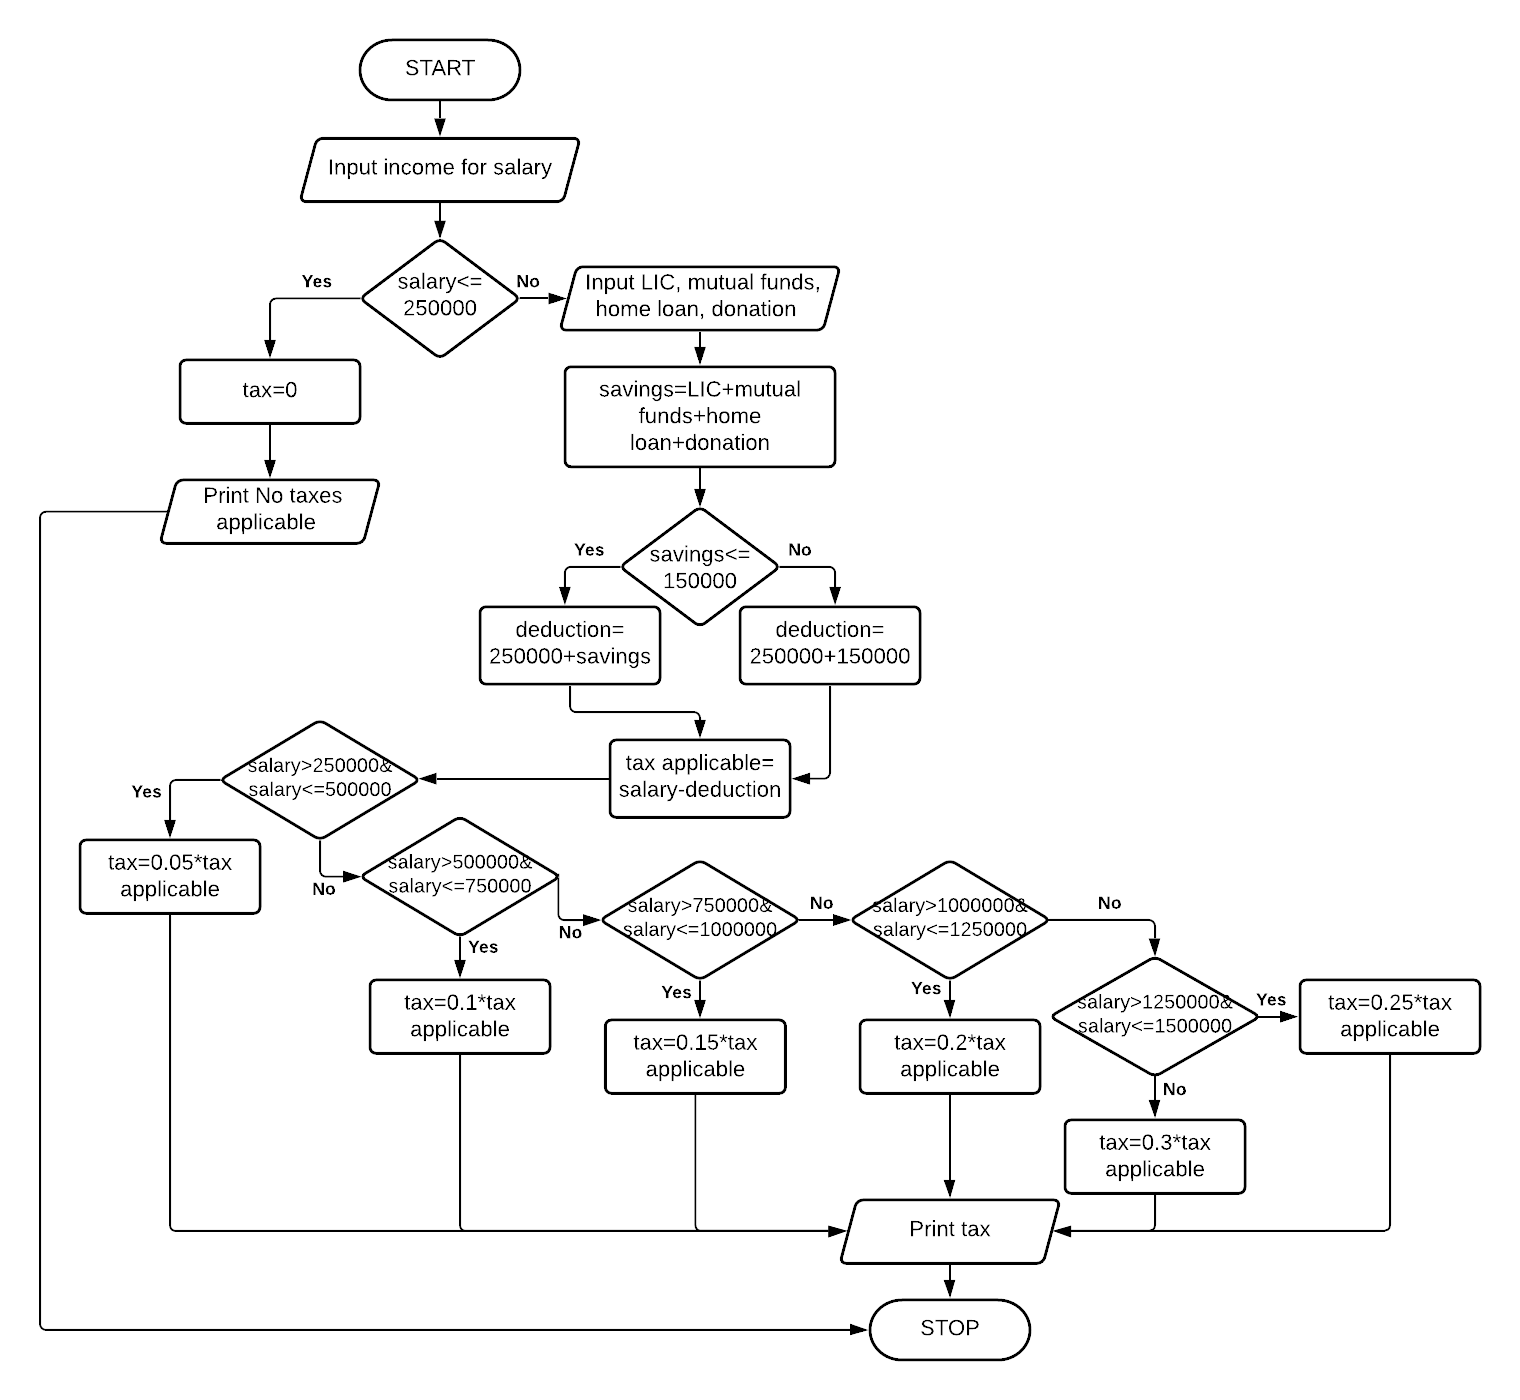
\includegraphics[width=1.1\textwidth]{Flowchart03.png}
\end{figure}
\newpage
\subsection{Code}
\inputminted{c}{q3.c}
\subsection{Output}
\begin{figure}[h]
    \centering
    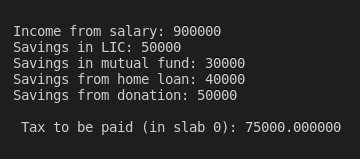
\includegraphics[width=0.5\textwidth]{3.png}
\end{figure}
\newpage
\section{}
\subsection{Flowchart}
\begin{figure}[h]
    \centering
    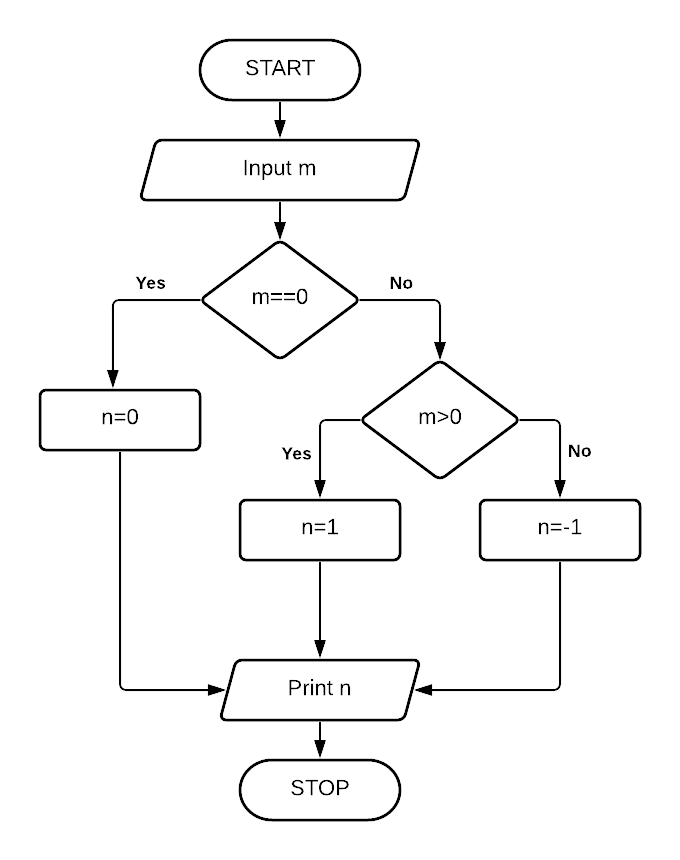
\includegraphics[width=0.6\textwidth]{Flowchart04.png}
\end{figure}
\newpage
\subsection{Code}
\inputminted{c}{q4.c}
\subsection{Output}
\begin{figure}[h]
    \centering
    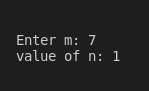
\includegraphics[width=0.5\textwidth]{4.png}
\end{figure}
\newpage
\section{}
\subsection{Flowchart}
\begin{figure}[h]
    \centering
    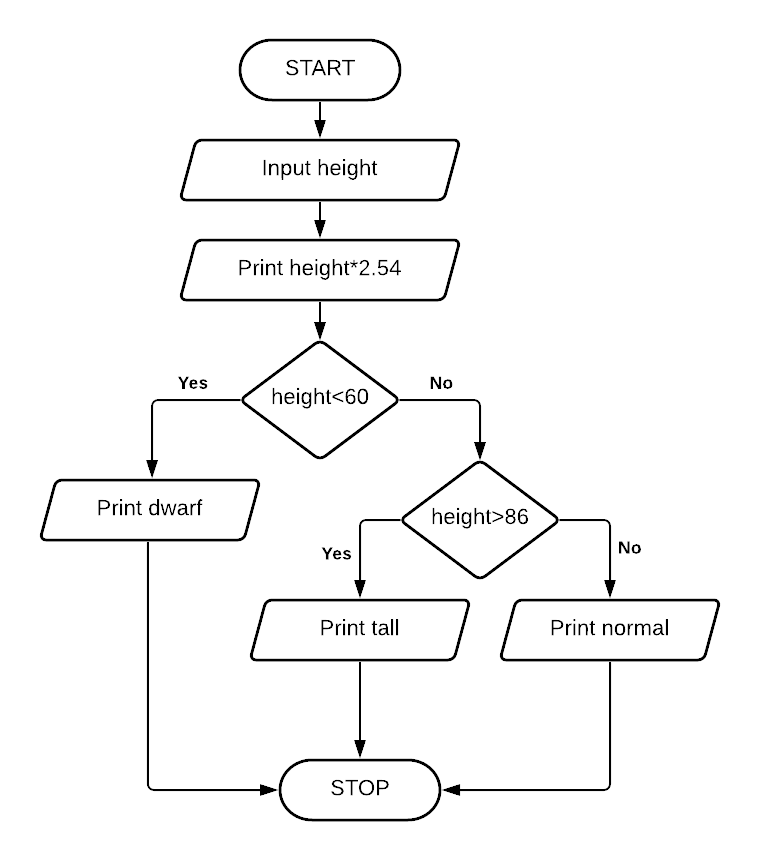
\includegraphics[width=0.8\textwidth]{Flowchart05.png}
\end{figure}
\newpage
\subsection{Code}
\inputminted{c}{q5.c}
\subsection{Output}
\begin{figure}[h]
    \centering
    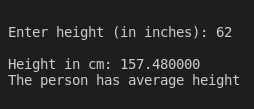
\includegraphics[width=0.5\textwidth]{5.png}
\end{figure}
\newpage
\section{}
\subsection{Flowchart}
\begin{figure}[h]
    \centering
    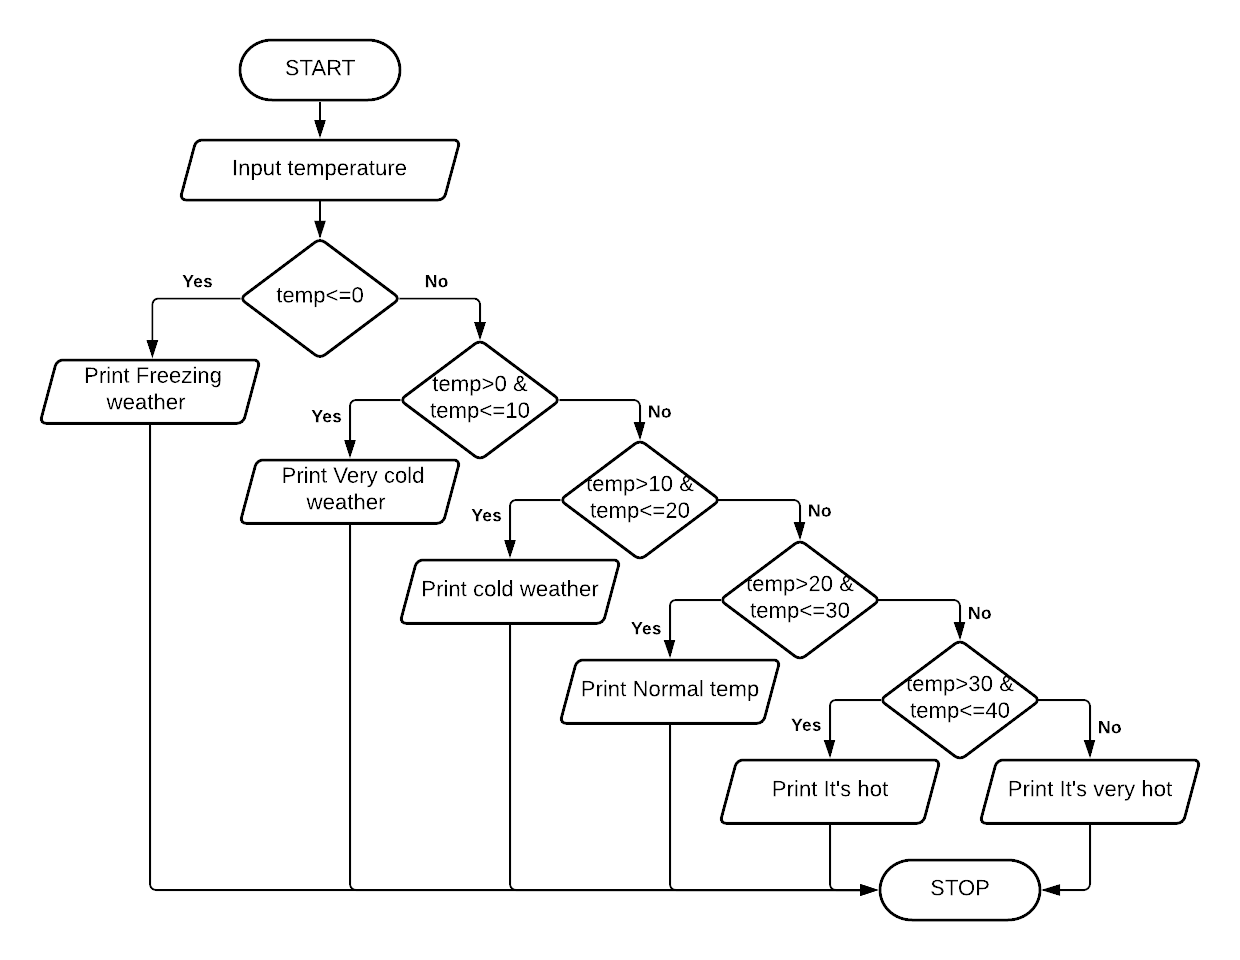
\includegraphics[width=1.1\textwidth]{Flowchart06.png}
\end{figure}
\newpage
\subsection{Code}
\inputminted{c}{q6.c}
\subsection{Output}
\begin{figure}[h]
    \centering
    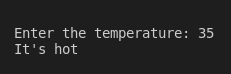
\includegraphics[width=0.5\textwidth]{6.png}
\end{figure}
\newpage
\section{}
\subsection{Flowchart}
\begin{figure}[h]
    \centering
    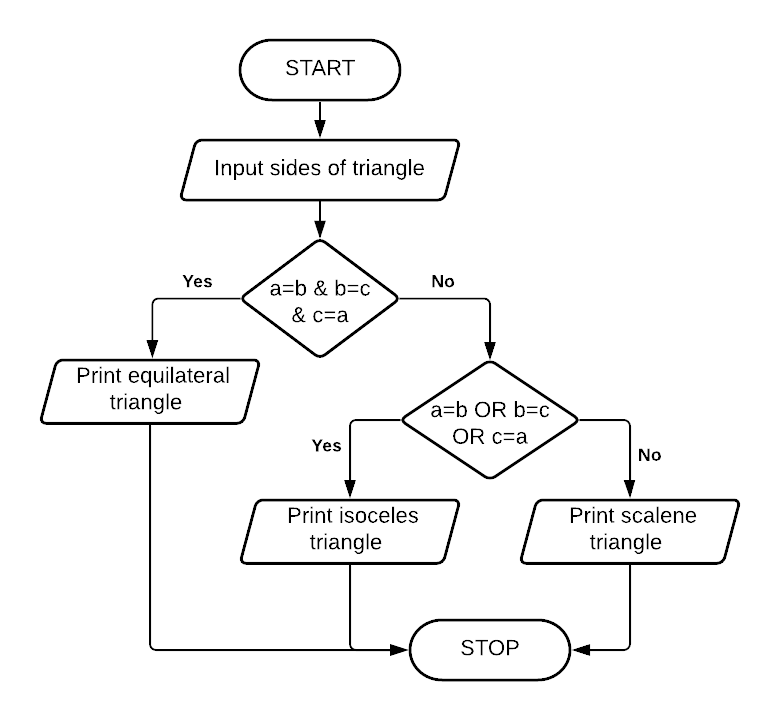
\includegraphics[width=1.0\textwidth]{Flowchart07.png}
\end{figure}
\newpage
\subsection{Code}
\inputminted{c}{q7.c}
\subsection{Output}
\begin{figure}[h]
    \centering
    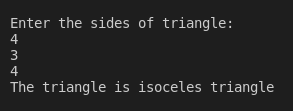
\includegraphics[width=0.5\textwidth]{7.png}
\end{figure}
\newpage
\section{}
\subsection{Flowchart}
\begin{figure}[h]
    \centering
    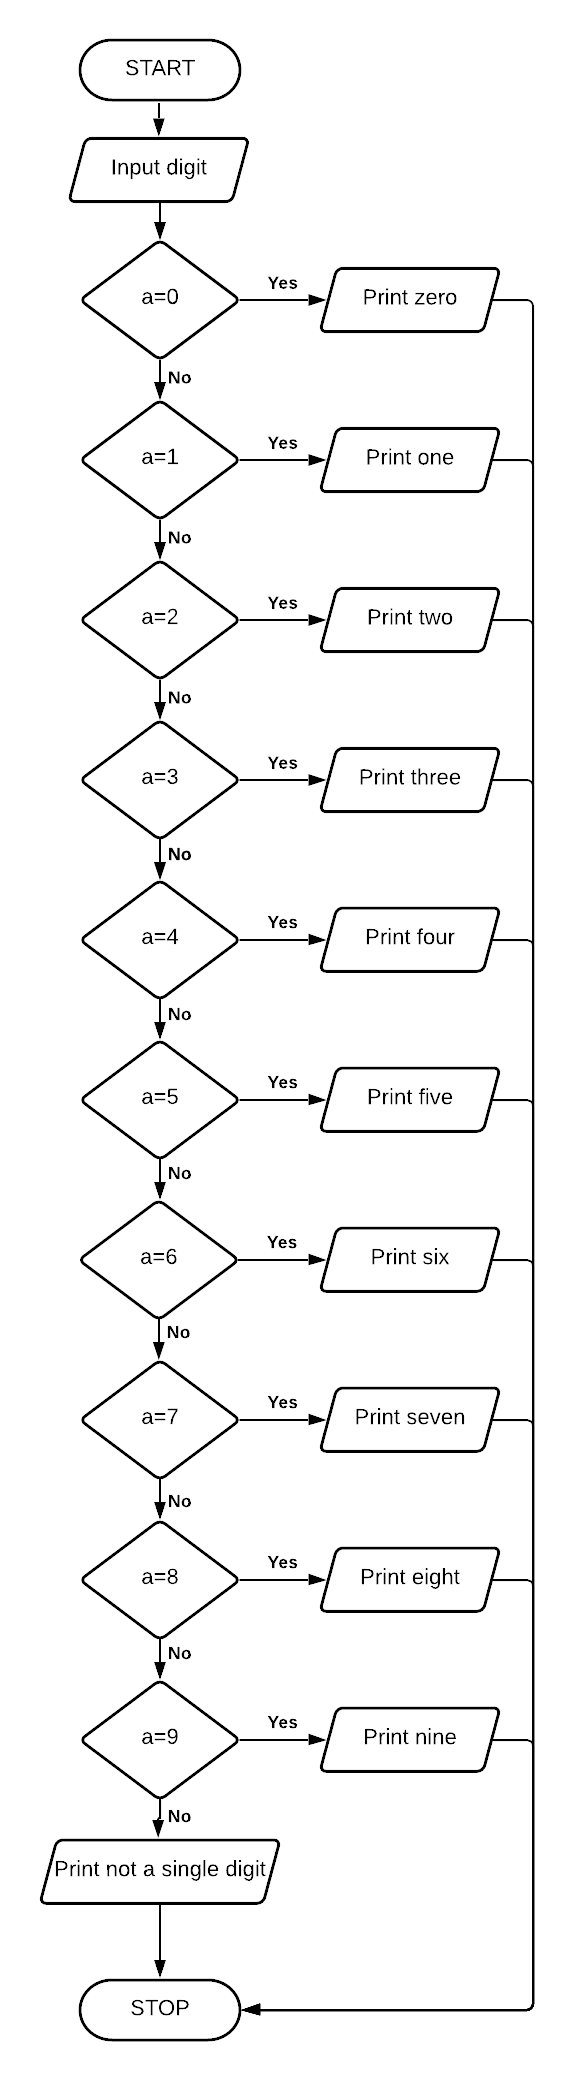
\includegraphics[width=0.3\textwidth]{Flowchart08.png}
\end{figure}
\newpage
\subsection{Code}
\inputminted{c}{q8.c}
\subsection{Output}
\begin{figure}[h]
    \centering
    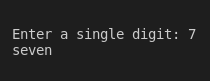
\includegraphics[width=0.5\textwidth]{8.png}
\end{figure}
\section{}
\subsection{Flowchart}
\begin{figure}[h]
    \centering
    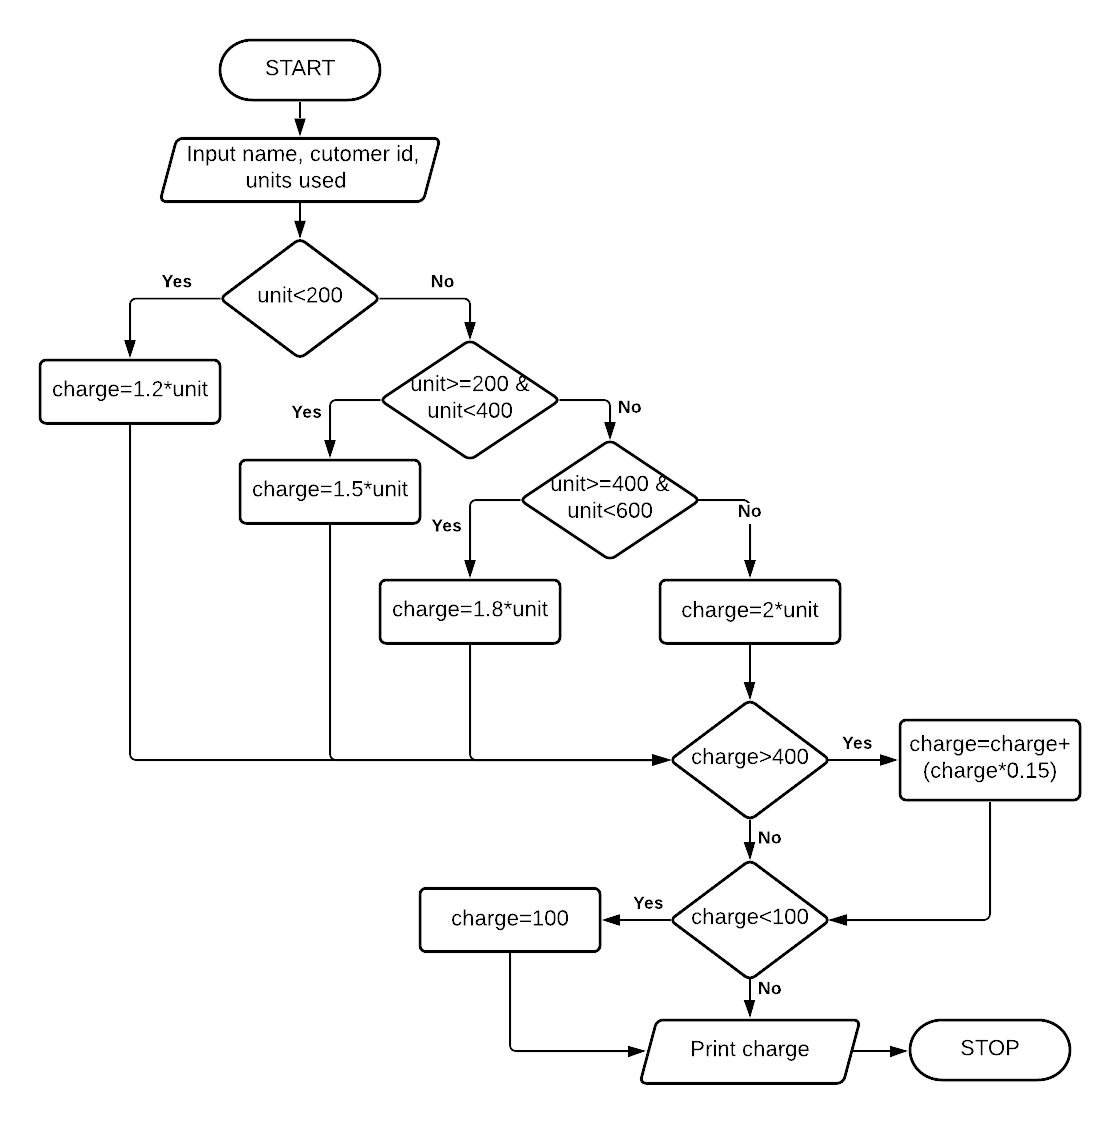
\includegraphics[width=0.85\textwidth]{Flowchart09.png}
\end{figure}
\newpage
\subsection{Code}
\inputminted{c}{q9.c}
\subsection{Output}
\begin{figure}[h]
    \centering
    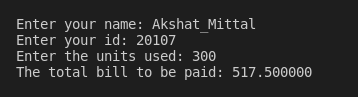
\includegraphics[width=0.7\textwidth]{9.png}
\end{figure}
\newpage
\section{}
\subsection{Flowchart}
\begin{figure}[h]
    \centering
    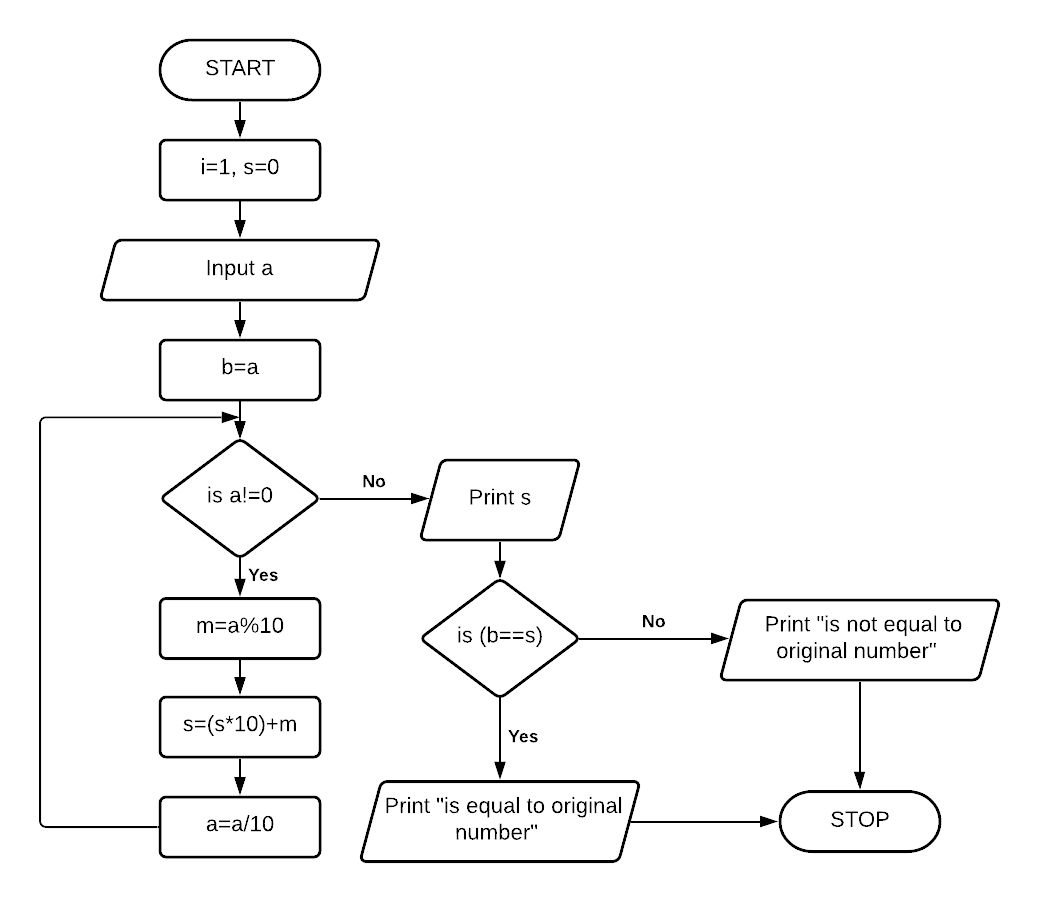
\includegraphics[width=1.0\textwidth]{Flowchart10.png}
\end{figure}
\newpage
\subsection{Code}
\inputminted{c}{q10.c}
\subsection{Output}
\begin{figure}[h]
    \centering
    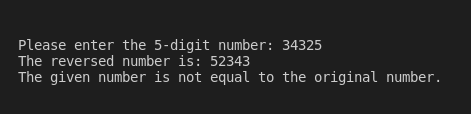
\includegraphics[width=0.8\textwidth]{10.png}
\end{figure}
\newpage
\end{document}